%Dokumentinformationen
\newcommand{\titleinfo}{Analysis An1E - Formelsammlung}
\newcommand{\authorinfo}{F. Braun, L. Schmid, U. Giger, R. Koller, C. Gwerder, S. K\"{o}rner, L. Leuenberger}
\newcommand{\versioninfo}{v1.5 / Januar 2013}

% standard header
%Schriftgr"osse, Layout, Papierformat, Art des Dokumentes
\documentclass[10pt,twoside,a4paper,fleqn]{article}
%Einstellungen der Seitenr"ander
\usepackage[left=1cm,right=1cm,top=1cm,bottom=1cm,includeheadfoot]{geometry}
% Sprache, Zeichensatz, packages
\usepackage[latin1]{inputenc}
\usepackage[ngerman]{babel,varioref}
\usepackage{amssymb,amsmath,fancybox,graphicx,color,lastpage,wrapfig,fancyhdr,hyperref,verbatim}

%pdf info
\hypersetup{pdfauthor={\authorinfo},pdftitle={\titleinfo},colorlinks=false}
%linkbordercolor=white
\author{\authorinfo}
\title{\titleinfo}

%Kopf- und Fusszeile
\pagestyle{fancy}
\fancyhf{}
%Linien oben und unten
\renewcommand{\headrulewidth}{0.5pt} 
\renewcommand{\footrulewidth}{0.5pt}

\fancyhead[L]{\titleinfo{ }\tiny{(\versioninfo)}}
%Kopfzeile rechts bzw. aussen
\fancyhead[R]{Seite \thepage { }von \pageref{LastPage}}
%Fusszeile links bzw. innen
\fancyfoot[L]{\footnotesize{\authorinfo}}
%Fusszeile rechts bzw. ausen
\fancyfoot[R]{\footnotesize{\today}} % ./header.tex nicht editieren (Projekt LaTeX-Header benutzen)

%%%%%%%%%%%%%%%%%%%%%%%%%%%%%%%%%%%%%%%%%%%%%%%%%%%%%%%%%%%%%%%%%%%%%%%%%%%%%%%%%%%%%%%%%%%%%%%%
% Neue Befehle und Definitionen                
%%%%%%%%%%%%%%%%%%%%%%%%%%%%%%%%%%%%%%%%%%%%%%%%%%%%%%%%%%%%%%%%%%%%%%%%%%%%%%%%%%%%%%%%%%%%%%%%
\definecolor{black}{rgb}{0,0,0}
\definecolor{red}{rgb}{1,0,0}
\definecolor{white}{rgb}{1,1,1}
\definecolor{grey}{rgb}{0.8,0.8,0.8}
\definecolor{lightgreen}{rgb}{0,1,0}
\definecolor{orange}{rgb}{1,0.549,0}
\definecolor{yellow}{rgb}{0.545,0.271,0.075}
\definecolor{violet}{rgb}{0.372,0.224,0.784}
\newcommand{\formelbuchgreen}[1]{$_{\textcolor{lightgreen}{\mbox{\small{S#1}}}}$}
\newcommand{\formelbuchred}[1]{$_{\textcolor{red}{\mbox{\small{S#1}}}}$}
\newcommand{\formelbuchorange}[1]{$_{\textcolor{orange}{\mbox{\small{S#1}}}}$}
\newcommand{\formelbuchyellow}[1]{$_{\textcolor{yellow}{\mbox{\small{S#1}}}}$}
\newcommand{\formelbuchviolet}[1]{$_{\textcolor{violet}{\mbox{\small{S#1}}}}$}

\begin{document}


%%%%%%%%%%%%%%%%%%%%%%%%%%%%%%%%%%%%%%%%%%%%%%%%%%%%%%%%%%%%%%%%%%%%%%%%%%%%%%%%%%%%%%%%%%%%%%%%
% Einführung                                   
%%%%%%%%%%%%%%%%%%%%%%%%%%%%%%%%%%%%%%%%%%%%%%%%%%%%%%%%%%%%%%%%%%%%%%%%%%%%%%%%%%%%%%%%%%%%%%%%
\section{Einf"uhrung}
\subsection{Zahlenmengen\formelbuchgreen{1,331}}
	\begin{minipage}[c]{6.5cm}
		$ \mathbb{N}  = \left\{1,2,3,...\right\};\; $\\
		$ \mathbb{Q} = \left\{x|x \;=\; ^{p}/_{q} \text{ mit } p \in \mathbb{Z}
		\text{ und } (q \in \mathbb{Z} \smallsetminus \{0\})\right\};\;$
	\end{minipage}
	\begin{minipage}[c]{5cm}
		$ \mathbb{N}_0  = \left\{0,1,2,3,...\right\};\; $\\
	\end{minipage}
	\begin{minipage}[c]{5cm}
		$ \mathbb{Z} = \left\{...,-2,-1,0,1,2,..\right\}; $\\
		$ \mathbb{R} = zB \; \sqrt{2}, \pi,\phi$
	\end{minipage}

\subsection{Mengenlehre\formelbuchgreen{334}}
	$A \;=\; \left\{-2,-1,0,1,2\right\} ,\; B\; =\; \left\{0,1,2,3,4\right\}$\\
	\begin{minipage}[c]{6.5cm}
		Schnittmenge:\\
		Vereinigungsmenge:\\
		Differenzmenge:\\
		Produktmenge:\\
		Kommutativgesetz:\\
		Assoziativgesetz:\\
		Distributivgesetz:
	\end{minipage}
	\begin{minipage}[c]{6.5cm}
		$A \; \cap  B \;=\;\left\{x|x \in A \text{ und } x \in B \right\}$\\
		$A \; \cup  B \;=\;\left\{x|x \in A \text{ oder } x \in B \right\}$\\			
		$A \; \smallsetminus B \;=\;\left\{x|x \in A \text{ und } x \notin B \right\}$\\
		$A \; \times B\;=\;\left\{(a,b)|a \in A \text{ und } b \in B \right\}$\\
		$A \; \cap  B \;=\;B \; \cap A$ \\
		$\left(A \cap  B \right) \cap C\;=\;A \cap \left( B \cap C \right)$ \\
		$A\; \cap \left(B\cup C\right)\;=\;\left(A \cup B\right)\cap \left(A \cup C\right) $ 
	\end{minipage}
	\begin{minipage}[c]{7cm}
		$A \; \cap B \;=\; \left\{0,1,2\right\}$\\
		$A \; \cup  B \;=\;\left\{-2,-1,0,1,2\right\}$\\
		$A \; \smallsetminus B \;=\;\left\{-2,-1\right\}$\\
		$ $\\
		$A \; \cup  B \;=\;B \; \cup A$ \\
		$\left(A \cup  B\right) \cup C\;=\;A \cup \left( B \cup C \right)$ \\
		$A\; \cup \left( B \cap C \right)\;=\;\left( A \cap  B \right) \cup \left(A \cap  C\right) $
	\end{minipage}
	
\subsection{Beweismethoden\formelbuchgreen{5}}

\subsection{Spezielle Ungleichungen\formelbuchgreen{30}}
	\begin{tabbing}	xxxxxxxxxxxxxxxxxxxxxxxxxxxxxxx\=xxxxxxxxxxxxxxxxxxxxxx\=xxxxxxxxxxxxxxxxxxxxxx\=xxxxxxxxxxxxxxxxxxxxxx\=\kill
		Bernoulli-Ungleichung: \>
			$(1 + a)^n > 1 + n \cdot a$\>
				f"ur $n \in N, n \geq 2, a \in R, a > -1, a\neq0$\\
		Binomische Ungleichung: \>
			$|a\cdot b|\leq\frac{1}{2}(a^2 + b^2)$\\
		Dreiecksungleichung: \>
			$\left|a+b\right|\leq\left|a\right|+\left|b\right|$ \>
				$\left|a-b\right|\leq\left|a\right|+\left|b\right|$ \>
					$\left|a-b\right|\geq\left|\left|a\right|-\left|b\right|\right|$\\
		Geometrisches und arithmetisches Mittel:\\ 
		f"ur $a_i\geq0,\;n \in \mathbb{N},\;i \in \left\{1,2,...,n \right\}:$\>
			$\sqrt[n]{a_1 a_2 \ldots a_n}\leq \frac{1}{n} \cdot \sum\limits _{i=1}^n a_i = 	\frac{a_1+a_2+...+a_n}{n}$\>\>
			$\sqrt{ab}\leq \frac{a+b}{2}$, siehe Br. S.19/20 \\
		Minima/Maxima: \>
			$\min\{a_i\} \leq \sqrt[n]{a_1a_2 \ldots a_n} \leq \max\{a_i\}$\\
		Betragsungleichung:\>$-c<x<c\;\Leftrightarrow\;|x|<c$
	\end{tabbing}

\subsection{Umgebung}
	\begin{minipage}[c]{14.5cm}
		Jedes offene Intervall, dass die Zahl a enth"alt, heisst eine Umgebung von a. \\
		Es sei $\epsilon >$ 0. Unter der $\epsilon$-Umgebung von a versteht man das offene Intervall $(a-\epsilon,a+\epsilon).$\\
		Eine $\epsilon$-Umgebung von a ohne die Zahl a selbst wird punktierte $\epsilon$-Umgebung von a genannt.
	\end{minipage}
	\begin{minipage}[c]{5cm}
	Schreibweise: U(a)\\
	Schreibweise: $U_\epsilon(a)$\\
	Schreibweise: $\dot{U}_\epsilon(a)=U_\epsilon(a)\smallsetminus{a}$
	\end{minipage}

\subsection{Summenzeichen\formelbuchgreen{7}}
	\begin{minipage}[c]{4.75cm}
		$\text{mit 1}\leq m\leq n $
	\end{minipage}
	\begin{minipage}[c]{16cm}
			Die Laufvariable $i$ wird immer um 1 aufaddiert. $i$ immer kleiner-gleich $n$ (z.B. wenn $i \in \mathbb{R}$)
	\end{minipage}
	\begin{minipage}[c]{4.75cm}
		$\sum\limits _{i=1}^n a_i = \sum\limits _{i=1}^m a_i + \sum\limits _{i=m+1}^n a_i;$
	\end{minipage}
	\begin{minipage}[c]{4.25cm}	
		$\sum\limits _{i=1}^n a_i = \sum\limits _{i=1-j}^{n-j} a_{i+j};$
	\end{minipage}
	\begin{minipage}[c]{4.25cm}
		$\sum\limits _{i=1}^n a = n\cdot a;$
	\end{minipage}
	\begin{minipage}[c]{8cm}
		$\sum\limits _{i=1}^n \left(\lambda a_i + \beta b_i \right) = $
		$\lambda \sum\limits _{i=1}^n a_i + \beta \sum\limits _{i=1}^n b_i$	
	\end{minipage}
	
\subsection{Spezielle endliche Reihen\formelbuchgreen{19}}
			\begin{minipage}[c]{4.25cm}
				$\sum\limits _{i=1}^n i = \frac{n(n+1)}{2}$
			\end{minipage}
			\begin{minipage}[c]{4.25cm}	
				$\sum\limits _{i=1}^n i^2 = \frac{n(n+1)(2n+1)}{6}$
			\end{minipage}
			\begin{minipage}[c]{4.25cm}
				$\sum\limits _{i=1}^n i^3 = \frac{n^2(n+1)^2}{4}$
			\end{minipage}

\subsection{Produktzeichen\formelbuchgreen{7}}
	$a_n\prod\limits _{i=1}^n \left(x-x_i\right)=
	a_n\cdot\left(x-x_1\right)\cdot\left(x-x_2\right)\cdot...\cdot\left(x-x_n\right)$
	
\subsection{Fakult"at\formelbuchgreen{13}}
	\begin{minipage}[c]{6cm}
		$n! = 1\cdot2\cdot3\cdot...\cdot n $
	\end{minipage}
	\begin{minipage}[c]{6cm}
		$\text{f"ur n} \in \mathbb{N}, n \geq 3$
	\end{minipage}
	\begin{minipage}[c]{6cm}
		$n!>2^{n-1}$
	\end{minipage}
	
\subsection{Binomischer Satz\formelbuchgreen{12}}
	\begin{minipage}[c]{6cm}
		$\left(a+b\right)^n = \sum\limits _{i=0}^n \left(\stackrel{n}{i}\right)a^{n-i}\cdot b^i$;\\
		$\left(\stackrel{n}{i-1}\right)+\left(\stackrel{n}{i}\right)=\left(\stackrel{n+1}{i}\right)$;
	\end{minipage}
	\begin{minipage}[c]{6cm}
		$\left(\stackrel{n}{i}\right)=\left(\stackrel{n}{n-i}\right)$\\
		$\left(\stackrel{n}{i}\right)=\frac{n!}{i!\left(n-i\right)!}$;
	\end{minipage}
	\begin{minipage}[c]{6cm}	
		$\left(\stackrel{n}{0}\right)=1$
	\end{minipage}
	
\subsection{Einige Wurzeln}
$\sqrt{2} = 1.414; \qquad \sqrt{3} = 1.732; \qquad \sqrt{5} = 2.236; \qquad \sqrt{6} = 2.449; \qquad \sqrt{7} = 2.645; \qquad \sqrt{8} = 2.828;$
%%%%%%%%%%%%%%%%%%%%%%%%%%%%%%%%%%%%%%%%%%%%%%%%%%%%%%%%%%%%%%%%%%%%%%%%%%%%%%%%%%%%%%%%%%%%%%%%%
%% Funktionen                                   
%%%%%%%%%%%%%%%%%%%%%%%%%%%%%%%%%%%%%%%%%%%%%%%%%%%%%%%%%%%%%%%%%%%%%%%%%%%%%%%%%%%%%%%%%%%%%%%%%
\begin{flushleft}
	\section{Funktionen\formelbuchred{48}}
		\subsection{Einleitung}
			\begin{minipage}[t]{5cm}
				\textbf{Schreibweisen:}\\
				$f:D_f \rightarrow W_f$ mit $x \mapsto f(x)$\\
				$f:x \mapsto f(x)$ mit $x \in D_f$\\
				$y=f(x)$ mit $x \in D_f$
			\end{minipage}
			\hfill
			\begin{minipage}[t]{8cm}
				\textbf{Definitionen:}\\
				$x \Rightarrow$ Argument oder Variable von $f$\\
				$f(x) \Rightarrow$ Funktionswert, Wert von $f$ an der Stelle $x$\\ 
				$x \mapsto f(x)$ oder $y=f(x) \Rightarrow$ Zuordnungsvorschrift\\
				$D_f \Rightarrow$ Definitonsmenge oder Definitionsbereich\\ 
				$W_f \Rightarrow$ Wertemenge oder Wertebereich
			\end{minipage}
			\hfill
			\begin{minipage}[t]{4cm}
				\textbf{Achsenbezeichnungen:}\\
				Abszisse = X-Achse\\
				Ordinate = Y-Achse\\
				Applikate = Z-Achse
			\end{minipage}	

		\subsection{Transformationen}
			\begin{minipage}[c]{5cm}
				$\mathbf{\pm \; {\color{red}a} \cdot f( \; \pm \; {\color{blue}b}x \; \pm \; 
				{ \; \color{green}c}) \; \pm \; {\color{cyan}d}}$\\
				 1.schieben 2.stecken\\
				$ $\\
				$\mathbf{\pm \; {\color{red}a} \cdot f( \; \pm \; {\color{blue}b} ( x \; \pm
				{ \; \color{green}c})) \; \pm \; {\color{cyan}d}}$\\
				1.strecken 2.schieben\\	
			\end{minipage}
			\begin{minipage}[t]{10cm}
				\begin{tabular}{lll}
					1. &\textbf{{\color{red}a}} &Vertikale (y-Richtung) Streckung um \textbf{a} bzw. Spiegelung an x bei \textbf{-a}\\
					2. &\textbf{{\color{blue}b}} &Horizontale (x-Richtung) Streckung um \textbf{1/b} bzw. Spiegelung an y bei \textbf{-b}\\
					3. &\textbf{{\color{green}c}} &Verschiebung nach links (\textbf{+c}) oder rechts (\textbf{-c}) (vertikale Verschiebung)\\
					4. &\textbf{{\color{cyan}d}} &Verschiebung nach oben (\textbf{+d}) oder unten (\textbf{-d}) (horizontale Verschiebung)
				\end{tabular}
			\end{minipage}
				
			\subsubsection{Spiegelung}
				an X-Achse: Polarit"at von $f$ "andern\\
				an Y-Achse: Polarit"at von $x$ "andern\\
			
		\subsection{Spezielle Funktionen}
			\begin{minipage}[t]{6cm}
				\textbf{Identit"at:}\\
				Schreibweise: $f(x)=x$\\\\
				Definition:\\
				Der X-Wert ist gleich dem Y-Wert
			\end{minipage}
			\hfill
			\begin{minipage}[t]{6cm}
				\textbf{Signumfunktion:}\\
				Schreibweise: $f(x)=sgn(x)$\\
				Definiton: $y=\left\{\begin{array}{l}\text{1, falls $x>0$}\\
				\text{0, falls $x=0$}\\\text{-1, falls $x<0$}\end{array}\right.$
			\end{minipage}	
			\hfill
			\begin{minipage}[t]{6cm}
				\textbf{Gauss-Klammer (floor):}\\
				Schreibweise: $f(x)=\left[x\right]$\\\\
				Definition:\\
				rundet den Y-Wert ganzzahlig ab
			\end{minipage}
				
		\subsection{Umkehrfunktion\formelbuchred{52}}
		\begin{tabbing}
			-----------------------------\= \kill
			Schreibweise: $f^{-1}$ \> Definition: ein Y-Wert darf nur einmal vorkommen und $W_f$ muss $\in D_f$ sein\\
			Ist eine Funktion $f$ auf einem Intervall $D$ streng monoton, dann existiert f"ur dieses Intervall die Umkehrfunktion $f^{-1}$
		\end{tabbing}
		
		\subsection{Verkettung oder mittelbare Funktion}
		\begin{tabbing}
			--------------------\=----------------------------------------------\=------------------\=-----------------\=----------------------\= \kill	
			Schreibweise: \> $h(x)=g \circ f \Rightarrow h(x)=g(f(x))$ \> Sprechweise: \> \textit{g nach f} \> Wertebereiche: \> $W_h=W_g \rightarrow D_h=D_f$\\
								    \> $h(x)=f \circ g \Rightarrow h(x)=f(g(x))$ \>  \> \textit{f nach g} \> \> $W_h=W_f \rightarrow D_h=D_g$
		\end{tabbing}
		
	 		\textbf{Wichtig:} Funktionen sind nacheinander ausf"uhrbar, wenn der $W_f \subset D_g$ bzw. $W_g \subset D_f$  ist.
			
		\subsection{Beschr"anktheit\formelbuchred{51}}
			
		\subsection{Monotonie\formelbuchred{50}}
			\begin{tabbing}
				-------------------------------------------------------------------------\= \kill
				\textbf{monoton wachsend} $\longrightarrow x_1<x_2 \Rightarrow f(x_1)\leq f(x_2)$\>
				\textbf{streng monoton wachsend} $\longrightarrow x_1<x_2 \Rightarrow f(x_1) < f(x_2)$\\
				\textbf{monoton fallend} $\longrightarrow x_1<x_2 \Rightarrow f(x_1)\geq f(x_2)$\>
				\textbf{streng monoton fallend} $\longrightarrow x_1<x_2 \Rightarrow f(x_1)>f(x_2)$
			\end{tabbing}		
\newpage
		\subsection{Gerade/Ungerade Funktionen\formelbuchred{51}}
			Funktion ist \textbf{gerade} wenn $f(-x)=f(x)\Rightarrow$ Achsensymmetrisch\\
			Funktion ist \textbf{ungerade} wenn $ f(-x)=-f(x)\Rightarrow \text{Punktsymmetrisch}$\\
			Funktion ist \textbf{periodisch} wenn $f(x) = f(x \pm p)\Rightarrow \text{wiederholt sich im Abstand p}$ \qquad
			$\text{f"ur beide gilt: } \underbrace{ x \in D_f \land -x \in D_f}_{D_f \text{ ist } \textbf{symmetrisch}}$\\
			\textbf{Wichtig:} Um zu beweisen das eine Funktion gerade bzw. ungerade ist, zeigt man indem man beweist, dass es f"ur \underline{einen} Punkt \underline{nicht} stimmt!\\
		
		\subsection{Ganzrationale Funktionen (Polynom)\formelbuchred{62,64}}
			Aussehen: \[f(x)=a_nx^{n}+a_{n-1}x^{n-1}+\cdots+a_1x+a_0\]\\
			Nullstellen bestimmen:\\
			\begin{itemize}
				\item falls Polynom ($ax^{2}+bx+c$) quadratische L"osungsformel: $\frac{-b\pm\sqrt{b^{2}-4ac}}{2a}$
				\item faktorisieren mit Hilfe von Binomen
				\item faktorisieren mit Hilfe des \textbf{Hornerschemas\formelbuchred{957}}
			\end{itemize}
			\textbf{Wichtig:} eine ganzrationale Funktion $n$-ten Grades hat h"ochstens $n$ verschiedene Nullstellen

		\subsection{Hornerschema\formelbuchred{965}}
			\begin{minipage}[t]{9cm}
				- Pfeile $\Rightarrow$ Multiplikation\\
				- Zahlen pro Spalte werden addiert\\
				\includegraphics[width=6cm]{./bilder/hornerschema_1.png}	\\
				$x_1 \Rightarrow$ Nullstelle (muss erraten werden, durch \textbf{ausprobieren}!!)\\
				oberste Zeile = zu zerlegendes Polynom			
			\end{minipage}
			\begin{minipage}[t]{9cm}
				\textbf{Beispiel:}\\
				$f(x) = x^3-67x-126$\\
				\includegraphics[width=6cm]{./bilder/hornerschema_2.png}\\
				$\Rightarrow f(x) = (x-x_1)(b_2x^2 + b_1x + b_0) = (x+2)(x^2-2x-63)$	
			\end{minipage}
			Ergebnis der Form: $f(x)=(x-x_1)(g(x)+f(x_1)\hspace*{1cm}$ Linearfaktor: $(x-x_1)\hspace*{1cm}$ Polynom vom Grad $n-1$: $g(x)$ \\
		
		\subsection{Gebrochenrationale Funktionen\formelbuchred{62,66}}
			Aussehen: \[f(x)=\frac{p_m(x)}{q_n(x)}=\frac{a_mx^{m}+a_{m-1}x^{m-1}+\cdots+a_1x+a_0}{a_nx^{n}+a_{n-1}x^{n-1}+\cdots+a_1x+a_0}\]\\
			Definitionen:\\
			\begin{itemize}
				\item wenn $m<n$ ist $f$ \textbf{echt gebrochen}, wenn $m\geq n$ ist $f$ \textbf{unecht gebrochen}\\
				\item $x_1$ ist \textbf{Nullstelle} von $f$ falls $p_m(x_1)=0$ und $q_n(x_1)\neq0$ gilt $\rightarrow$ k-fache Nullstelle\\
				\item $x_1$ heisst \textbf{Polstelle} von $f$ falls $q_n(x_1)=0$ und $p_m(x_1)\neq0$ gilt $\rightarrow$ k-fache Polstelle\\
				\item $x_1$ heisst \textbf{L"ucke} von $f$ falls $q_n(x_1)=0$ und $p_m(x_1)=0$ gilt.\\
				\item Jede unecht gebrochene rationale Funktion l"asst sich als Summe einer ganzrationalen Funktion und einer echt gebrochenen Funktion
							schreiben. Dies ist m"oglich mit der \textbf{Polynomdivision\formelbuchred{15}}
			\end{itemize}			
			
		\subsection{Partialbruchzerlegung\formelbuchred{15}}
			\[f(x)=\frac{x^2+20x+149}{x^3+4x^2-11x-30} \Rightarrow \; \begin{array}{l}\text{Nenner faktorisieren mit}\\
			\text{Hornerschema\formelbuchred{965}, Binom}\end{array} \Rightarrow x^{3}+4x^{2}-11x-30=(x+2)(x^{2}+2x-15)=(8x+2)(x+5)(x-3)\]
			Ansatz:
			\[f(x)=\frac{x^2+20x+149}{x^3+4x^2-11x-30}=\frac{A}{x-3} + \frac{B}{x+2} + \frac{C}{x+5}=
			\frac{A(x+2)(x+5)+B(x-3)(x+5)+C(x-3)(x+2)}{(x-3)(x+2)(x+5)}\]
			Gleichungssystem \textbf{(Z"ahler gleichsetzen)} aufstellen mit beliebigen $x_i$-Werten (am Besten Polstellen oder 0,1,-1 w"ahlen):
			\[\begin{array}{l}x_1=3:\;-9+60+149=A\cdot5\cdot8\;\;\;\Rightarrow A=5\\
			x_2=-2:\;-4-40+149=B(-5)\cdot3\; \Rightarrow B=-7\\
			x_3=-5:\;-25-100+149=C(-8)(-3) \Rightarrow C=1 \end{array} \Rightarrow f(x)=\frac{5}{x-3}+\frac{7}{x+2}\frac{1}{x+5}\]
			weitere Ans"atze f"ur andere Typen von Termen: (Mehrere Werte f"ur $x$ verwenden, auch wenn kein Koeffizient 0 wird.)
			\[f(x)=\frac{5x^2-37x+54}{x^3-6x^2+9x}=\frac{A}{x}+\frac{B}{x-3}+\frac{C}{(x-3)^2}=\frac{A(x-3)^2+Bx(x-3)+Cx}{x(x-3)^2}\]
			\[f(x)=\frac{1,5x}{x^3-6x^2+12x-8}=\frac{A}{x-2}+\frac{B}{(x-2)^2}+\frac{C}{(x-2)^3}=\frac{A(x-2)^2+B(x-2)+C}{(x-2)^3}\]
			\[f(x)=\frac{x^2-1}{x^3+2x^2-2x-12}=\frac{A}{x-2}+\frac{Bx+C}{x^2+4x+6}=\frac{A(x^2+4x+6)+(Bx+C)(x-2)}{(x-2)(x^2+4x+6)}\]
							
		\subsection{Trigonometrische Funktionen\formelbuchred{76ff} Arcus\formelbuchred{86}}
			\begin{tabbing}
				-----------------------------------------------------------------\= \kill
				$\sin: D_f=[-\frac{\pi}{2},\frac{\pi}{2}]\rightarrow W_f=[-1,1]$ \> $\arcsin: D_f=[-1,1]\rightarrow W_f=[-\frac{\pi}{2},\frac{\pi}{2}]$\\
				$\cos: D_f=[0,\pi]\rightarrow W_f=[-1,1]$ \> $\arccos: D_f=[-1,1]\rightarrow W_f=[0,\pi]$\\
				$\tan: D_f=(-\frac{\pi}{2},\frac{\pi}{2})\rightarrow W_f=\mathbb{R}$ \> $\arctan: D_f=\mathbb{R}\rightarrow W_f=(-\frac{\pi}{2},\frac{\pi}{2})$\\
				$\cot: D_f=(0,\pi)\rightarrow W_f=\mathbb{R}$ \> arccot: $D_f=[-1,1]\rightarrow W_f=(0,\pi)$\\											
				Orthogonalit"atsbedingung: $m_1 \cdot m_2 = -1$
			\end{tabbing}


		\subsection{Schwingungen\formelbuchred{83}}

		\subsection{Potenz- und Wurzelfunktionen\formelbuchred{8,71}}
			\textbf{gerade Potenzfunktion:} $D_f=\mathbb{R} \rightarrow W_f=\mathbb{R}^+_0\;\;$
			\textbf{ungerade Potenzfunktion:} $D_f=\mathbb{R} \rightarrow W_f=\mathbb{R}$\\		
			\textbf{gerade Wurzelfunktion:} $D_f=\mathbb{R}^+ \rightarrow W_f=\mathbb{R}\;\;$
			\textbf{ungerade Wurzelfunktion:} $D_f=\mathbb{R} \rightarrow W_f=\mathbb{R}$
		
		\subsection{Hyperbolische Funktionen\formelbuchred{88} Areahyperbolicus\formelbuchred{92}}
			$	\sinh(x)=\frac{e^x-e^{-x}}{2}; D=\mathbb{R}, W=\mathbb{R} $
			\hspace{1.2cm}
			$ \cosh(x)=\frac{e^x+e^{-x}}{2}; D=\mathbb{R}, W=[1,\infty ) $
			\hspace{1.2cm}
			$ \tanh(x)=\frac{e^x-e^{-x}}{e^x+e^{-x}}; D=\mathbb{R}, W=(-1,1)  $
		
		\subsection{Logarithmus- und e-Funktion\formelbuchred{9,72}}
			\begin{minipage}[c]{9cm}
				\textbf{e-Funktion:} 
				$D_f=\mathbb{R} \rightarrow W_f=\mathbb{R}^+$ \\ \\
				%%$$e^x=\lim_{n \to \infty} (1+\frac{x}{n})^n$$				
				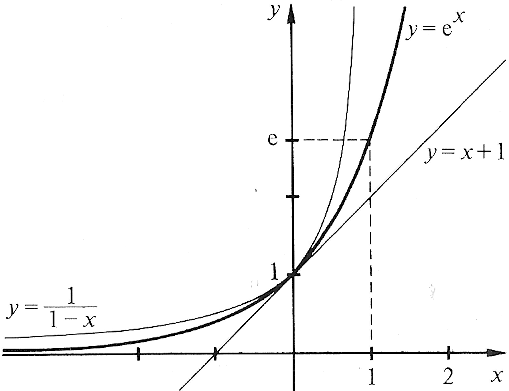
\includegraphics[height=4cm]{./bilder/funktionen_e.png} \\ \\
				$e^x \geq 1+x$ f"ur $x \in \mathbb{R}$\\
				$e^x \leq \frac{1}{1+x}$ f"ur $x < 1$\\
				$e=\lim\limits_{n\rightarrow\infty}(1+\frac{1}{n})^n$\\
			\end{minipage}
			\begin{minipage}[c]{9cm}
				\textbf{Logartihmus-Funktion:} $D_f=\mathbb{R}^+ \rightarrow W_f=\mathbb{R}$ \\ \\
				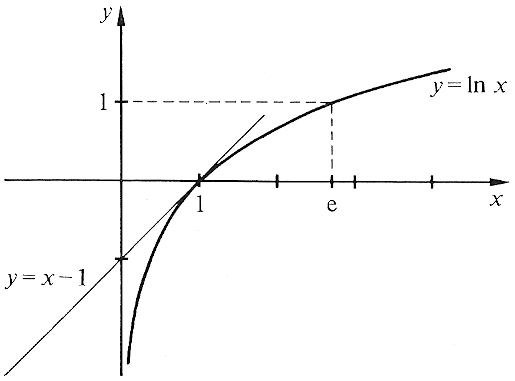
\includegraphics[height=4cm]{./bilder/funktionen_ln.png}\\
				$1-\frac{1}{x} \leq ln(x) \leq x-1$
			\end{minipage}
	
		\subsection{$\varepsilon - M$ - Kriterium\formelbuchred{53}}
			$|f(x) - g| < \varepsilon$ f"ur alle $x \geq M(\varepsilon)$

		\subsection{$\varepsilon - \delta$ - Kriterium\formelbuchred{53}}
			$|f(x) - g| < \varepsilon \qquad 0 < |x - x_0| < \delta(\varepsilon) \qquad \text{f"ur } x \rightarrow x_0$
	
		\subsection{K-Kriterium\formelbuchred{54}}
			$f(x) > K$ f"ur $x > M$, $K \in \mathbb{R}$\\
			$f(x) < k$ f"ur $x < m$, $ k \in \mathbb{R}$

\end{flushleft}

%%%%%%%%%%%%%%%%%%%%%%%%%%%%%%%%%%%%%%%%%%%%%%%%%%%%%%%%%%%%%%%%%%%%%%%%%%%%%%%%%%%%%%%%%%%%%%%%%
%% Zahlenfolgen und Grenzwerte                  
%%%%%%%%%%%%%%%%%%%%%%%%%%%%%%%%%%%%%%%%%%%%%%%%%%%%%%%%%%%%%%%%%%%%%%%%%%%%%%%%%%%%%%%%%%%%%%%%%
\section{Zahlenfolgen\formelbuchorange{18,469}}
\subsection{Einf"uhrung\formelbuchorange{18}}

\begin{minipage}[c]{5cm}
	arithmetische Folge: \\
	$a_1=c$ und $a_{n+1}=a_n+d$ \\
	\\
	geometrische Folge:\\
	$a_1=c$ und $a_{n+1}=q*a_n$\\
\end{minipage}
\begin{minipage}[c]{2.5cm}
	$ $\\
	$\underbrace{d=a_{n+1}-a_n}_{Differenz}$\\
	$ $\\
	$\underbrace{q=\frac{a_{n+1}}{a_n}}_{Quotient}$
\end{minipage}
\begin{minipage}[c]{10cm}	
	\begin{tabular}{|c|c|c|c|}
		\hline
		\multicolumn{4}{|c|}{Monotonie} \\
		\hline
		$d \geq 0$ & $q \geq 1$ & monoton wachsend & $\uparrow$\\
		\hline
		$d > 0$ & $q > 1$ & streng monoton wachsend & $\Uparrow$\\
		\hline
		$d \leq 0$  & $0 < q \leq 1$ & monoton fallend & $\downarrow$\\
		\hline
		$d < 0$ & $0 < q < 1$ & streng monoton fallend & $\Downarrow$\\
		\hline
	\end{tabular}
\end{minipage}
	\\
	konstante Folge:\\
	$a_1=c$ und $a_{n+1}=c$

\subsection{Beschr"anktheit\formelbuchorange{51,469}}
	$\text{Beschr"ankt wenn }k\leq a_n\leq\text{ K,	wobei k bzw. K die untere bzw. obere Schranke
	ist}$
\subsubsection{Bolzano-Weierstrass}
	Jede beschr"ankte und monotone Zahlenfolge ist konvergent.

\subsection{Grenzwerts"atze\formelbuchorange{470}}

\subsection{Grenzwerte von rekursiven Folgen}

\begin{flushleft}
\begin{enumerate}
	\item Hypothetischer Grenzwert ausrechnen \\[5pt]
		\begin{minipage}[t]{4.5cm}
			$  \lim\limits_{n\rightarrow\infty} a_n = \lim\limits_{n\rightarrow\infty} a_{n+1} = a $
			\end{minipage}
			\begin{minipage}[t]{12cm}
			$\text{z.B.}\sqrt{a_n}+1=a_{n+1}\Rightarrow\lim\limits_{n\rightarrow\infty}\;\sqrt{a}+1 = a$\\
			$\Rightarrow x=\frac{3\pm\sqrt{5}}{2}\Rightarrow$ M"oglicher Grenzwert $\rightarrow$ wenn Folge beschr"ankt und monoton 
			\end{minipage}\\[5pt]	

	\item Beschr"anktheit mittels des hypothetischen Grenzwertes\\
$\Rightarrow$ mit vollst"andider Induktion beweisen (Auch mit Ungleichungen l"osbar)\\
			\begin{minipage}[t]{20cm}
				\begin{minipage}[t]{1cm}
					z.B.
				\end{minipage}
				\begin{minipage}[t]{5cm}
					Induktionsanfang $A(1)$:\\
					Induktionsschritt $A(n+1)$:\\
				\end{minipage}
				\begin{minipage}[t]{15cm}
					$a_1 < \frac{3+\sqrt{5}}{2} < 3 \Rightarrow 1 < 3 $\\
					$a_n < 3$ \hspace{5cm}$|\sqrt{...}\quad |+1$\\
					$\underbrace{\sqrt{a_n}+1}_{a_{n+1}} < \sqrt{3}+1 < 3$\\
				\end{minipage}   
			\end{minipage}  



	\item Monotonie annehmen (ev. erste Glieder berechnen)\\
		$\Rightarrow$ mit vollst"andiger Induktion beweisen (Auch mit q/d-Kriterium oder Ungleichungen l"osbar)\\
			\begin{minipage}[t]{20cm}
				\begin{minipage}[t]{1cm}
					z.B.
				\end{minipage}
				\begin{minipage}[t]{5cm}
					Induktionsanfang $A(1)$:\\
					Induktionsschritt $A(n+1)$:\\
				\end{minipage}
				\begin{minipage}[t]{15cm}
					$a_1 < a_2 \Rightarrow 1 < 2 $\\
					$a_n < a_{n+1}$ \hspace{5cm}$|\sqrt{...}\quad |+1$\\
					$\underbrace{\sqrt{a_n}+1}_{a_{n+1}} < \underbrace{\sqrt{a_{n+1}}+1}_{a_{n+2}}$\\
				\end{minipage}   

			\end{minipage}  
            \item Grenzwert bestimmen\\
		$\Rightarrow$ Aus 2. und 3. folgt das $x=\frac{3+\sqrt{5}}{2}\rightarrow$ Da Folge nach oben beschr"ankt und streng monoton wachsend
\end{enumerate}
					



\subsection{$\varepsilon - n_0$ - Kriterium\formelbuchorange{470}}
	$|a_n - a| < \varepsilon$ f"ur alle $n \geq n_0(\varepsilon)$

\end{flushleft}

%%%%%%%%%%%%%%%%%%%%%%%%%%%%%%%%%%%%%%%%%%%%%%%%
% Grenzwerte von Funktionen, Stetigkeit        
%%%%%%%%%%%%%%%%%%%%%%%%%%%%%%%%%%%%%%%%%%%%%%%%
\section{Grenzwerte von Funktionen\formelbuchorange{53}}

	\subsection{Berechnung von Grenzwerten\formelbuchorange{56}}
		Technik des $Erweiterns$: $\lim\limits_{n\to\infty} \frac{n}{n^2}$
		$\Longrightarrow $ Erweitern mit
		$\frac{1}{n^2} \Longrightarrow \lim\limits_{n\to\infty}$
		$\frac{\frac{n}{n^2}}{\frac{n^2}{n^2}} =$
		$\lim\limits_{n\to\infty} \frac{1}{n} = 0 $\\\\
		$Binomische Formel$: $\quad\lim\limits_{n\to\infty}\sqrt{n+1}-\sqrt{n} =$ 
		$\lim\limits_{n\to\infty} $
		$\frac{(\sqrt{n+1}-\sqrt{n})(\sqrt{n+1}+\sqrt{n})}{\sqrt{n+1}+\sqrt{n}} = $
		$\lim\limits_{n\to\infty} \frac{n+1-n}{\sqrt{n+1}+\sqrt{n}}= 0$

	\subsubsection{Spezielle Grenzwert S"atze}
		\begin{minipage}[t]{6 cm}
			$\lim\limits_{x\to x_0} |f(x)| = |\lim\limits_{x\to x_0} f(x)| = |g|$\\
		\end{minipage}
		\begin{minipage}[t]{6 cm}
			$\lim\limits_{x\to x_0} (f(x))^n = (\lim\limits_{x\to x_0} f(x))^n = g^n$ \\
		\end{minipage}
		\begin{minipage}[t]{6 cm}
			$\lim\limits_{x\to x_0} \sqrt[n]{f(x)} = \sqrt[n]{\lim\limits_{x\to x_0} f(x)} = \sqrt[n]{g}$
		\end{minipage}

	\subsubsection{Einschliessungsprinzip\formelbuchorange{55}}
		\begin{minipage}[t]{9 cm}
			$\lim\limits_{n \to \infty} a_n = \lim\limits_{n \to \infty} b_n = g \wedge a_n, b_n$ sind konvergent\\
		\end{minipage}
		\begin{minipage}[t]{9 cm}
			$a_n \leq c_n \leq b_n \Rightarrow \lim\limits_{n \to \infty} c_n = g$
		\end{minipage}

	\begin{figure}[ht]
		\begin{minipage}[b]{10.4 cm}
			\subsection{Links-/Rechtsseitiger Grenzwert\formelbuchorange{54}}
				Rechtsseitiger Grenzwert: $\lim\limits_{x \to x_0^+} f(x) = \lim\limits_{x \downarrow x_0}$
				$f(x) = g^+$\\
				Linksseitiger Grenzwert: $\lim\limits_{x \to x_0^-} f(x) = \lim\limits_{x \uparrow x_0}$
				$f(x) = g^-$

			\subsection{Konvergenz, Divergenz\formelbuchorange{474}}
				Konvergenz: $g^+ = g^- = g \in \mathbb{R}$ oder: monoton und beschr"ankt\\
				Bestimmte Divergenz: $g = +\infty$ oder: $g = -\infty$\\ 
				Unbestimmte Divergenz: Es existiert kein Grenzwert\\
				\small{($g$ f"ur Grenzwert)}

			\subsection{Stetigkeit\formelbuchorange{59}}
				"`Wenn man die Funktion mit einem Strich zeichnen kann"':\\
				$\lim\limits_{x \to x_0} f(x) = f(x_0)$
  		\end{minipage}
  		\begin{minipage}[b]{8 cm}
    		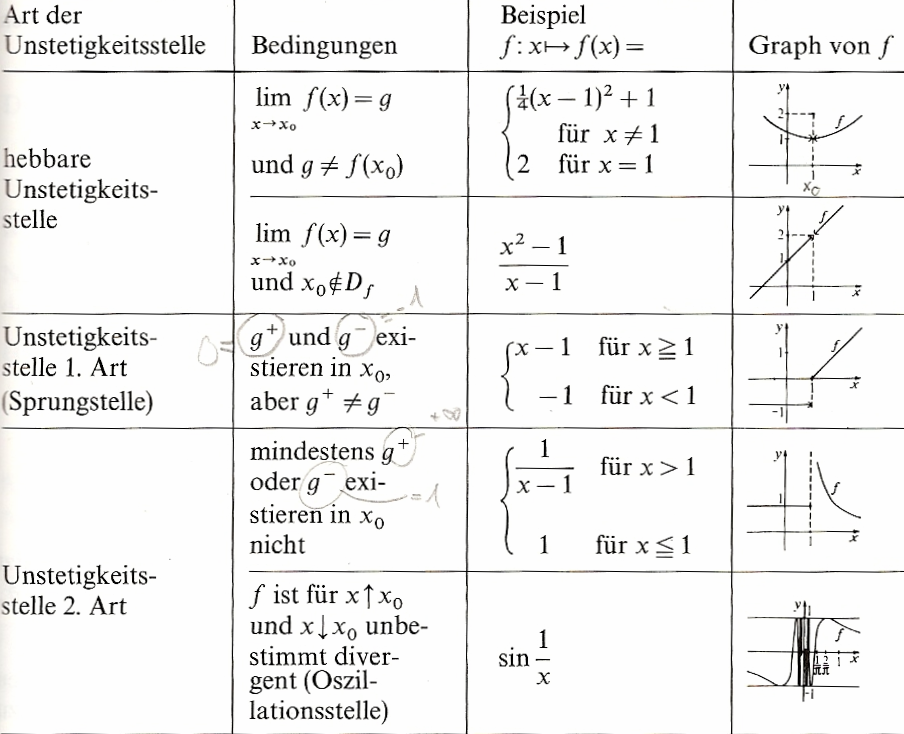
\includegraphics[width=8 cm]{./bilder/grenzwerte_unstetigkeitsstellen.png}
  		\end{minipage}
	\end{figure}
	
	\subsection{"Ubertragungsprinzip}
				\begin{tabbing}
		--------\=---------------------------------------------------\=---------------------------------------------------\=---------------------------------------------------\=\kill
			$f$ besitzt genau an der Stelle $x_0$ den Grenzwert $g$, wenn f"ur jede gegen $x_0$ konvergente Folge $<x_n>$ gilt: $\lim\limits_{n\to\infty}f(x_n)=g$\\
			Bsp: \>
			$f(x)=x-[x]$ und $x_0=-1$\>
			$x_n=-1-\frac{1}{n} \rightarrow \lim\limits_{n\to\infty}(x_n)=-1$\>
			$x_n'=-1+\frac{1}{n} \rightarrow \lim\limits_{n\to\infty}(x_n')=-1$\\	
			\>wenn nun gilt\\
			\>$\lim\limits_{n\to\infty}f(x_n)=\lim\limits_{n\to\infty}(-1-\frac{1}{n}-[-1-\frac{1}{n}])=1\neq\lim\limits_{n\to\infty}f(x_n')=\lim\limits_{n\to\infty}(-1+\frac{1}{n}-[-1+\frac{1}{n}])=0$\\
			\>Dann besitzt die Funktion $f(x)$ an der Stelle $x_0$ keinen Grenzwert $g$.
		\end{tabbing}

	\subsection{Spezielle Grenzwerte\formelbuchorange{58}}
  		\begin{minipage}[c]{6.33cm}
			$\lim\limits_{x \to 0} \frac{\sin{x}}{x} = 1 $
  		\end{minipage}
  		\begin{minipage}[c]{6.33cm}
			$ \lim\limits_{x \to \infty} \frac{x^{\alpha}}{a^{\beta x}} = 0 \:(a>1;\:\alpha, \beta > 0 ) $
  		\end{minipage}
  		\begin{minipage}[c]{6.33cm}
			$ \lim\limits_{x \to \infty} \frac{x^\alpha}{a^{\beta x}} = 0 $
  		\end{minipage} \\ \\
  		\begin{minipage}[c]{6.33cm}
			$ \lim\limits_{x \to \infty} (1+\frac{a}{x})^x=e^a $
  		\end{minipage}
  		\begin{minipage}[c]{6.33cm}
			$ \lim\limits_{x \to 0} (1+x)^{\frac{1}{x}}=e $
  		\end{minipage}
  		\begin{minipage}[c]{6.33cm}
				$ \lim\limits_{x \to 0} \frac{a^x-1}{x}=\ln a $
  		\end{minipage} \\ \\
  		\begin{minipage}[c]{6.33cm}
				$ \lim\limits_{x \to 0} \frac{\log_a(x+1)}{x} = \frac{1}{\ln a} $
  		\end{minipage}
  		\begin{minipage}[c]{6.33cm}
			$ \lim\limits_{x \to \infty} \frac{(\ln x)^\alpha}{x^{\beta}} = 0 $
  		\end{minipage}
  		\begin{minipage}[c]{6.33cm}
			$ \lim\limits_{x \to 2} \ln{\sqrt{\frac{x^2-4}{x-2}}} = \ln{2} $
  		\end{minipage} \\ \\
  		\begin{minipage}[c]{6.33cm}
			$ \lim\limits_{x \to 1} \frac{\ln{x}}{x-1} = 1 $
  		\end{minipage}
  		\begin{minipage}[c]{6.33cm}
			$ \lim\limits_{x \to 0+} x \ln{x} = 0 $
  		\end{minipage}
  		\begin{minipage}[c]{6.33cm}
			$ \lim\limits_{x \to 0} \frac{e^x-1}{x}=1 $
  		\end{minipage} \\ \\
  		\begin{minipage}[c]{6.33cm}
			$ \lim\limits_{x \to 0} \frac{x}{1-e^{-x}}=1 $
  		\end{minipage}
  		\begin{minipage}[c]{6.33cm}
			$ \lim\limits_{x \to \infty} \sum_{k=0}^n q^k = \begin{cases}+\infty &q \geq 1\\ \frac{1}{1-q} &|q|<1\end{cases} $
  		\end{minipage}
  		\begin{minipage}[c]{6.33cm}
			$ \lim\limits_{\alpha \to 0} \frac{(1+x)^{\alpha}-1}{x} = \alpha $
  		\end{minipage} \\ \\
  		\begin{minipage}[c]{6.33cm}
			$ \lim\limits_{x \to \infty} \frac{x^n}{n!} = 0 \:(x>0) $
  		\end{minipage}
  		\begin{minipage}[c]{6.33cm}
			$ \lim\limits_{x \to \infty} \frac{x^k}{q^x}=0 \:(q>1; \:k\in \mathbb{N}) $
  		\end{minipage}
  		\begin{minipage}[c]{6.33cm}
			$ \lim\limits_{x \to \infty} \sqrt[x]{p}=1 $
  		\end{minipage} \\ \\
  		\begin{minipage}[c]{6.33cm}
			$ \lim\limits_{x \to \infty} \sqrt[x]{x}=1 $
  		\end{minipage}

	\subsection{Asymptotenbestimmung\formelbuchorange{15}}
		Ausrechnen der Asymptote einer gebrochen rationalen Funktion $r: x \mapsto r(x)=\frac{P_m(x)}{Q_n(x)}$:
		\begin{tabbing}
		-----------------------------------\=-----------------------------------\=-----------------------------------\=\kill
			\>$m < n$ \>$m=n$ \>$m > n$\\
			$\lim\limits_{x\to \pm \infty} r(x) = $ 
			\>0 \>$\frac{a_m}{b_n}$ \> $+\infty$ oder $-\infty$\\
			Asymptote 
			\>x-Achse \>Parallel zur x-Achse \>Ganzrationaler Teil\\
			\> \>$y = g(x) = \frac{a_m}{b_n}$ \>der Polynomdivision\formelbuchorange{15}
		\end{tabbing}
%%%%%%%%%%%%%%%%%%%%%%%%%%%%%%%%%%%%%%%%%%%%%%%%%%%%%%%%%%%%%%%%%%%%%%%%%%%%%%%%%%%%%%%%%%%%%%%%
% Differential
%%%%%%%%%%%%%%%%%%%%%%%%%%%%%%%%%%%%%%%%%%%%%%%%%%%%%%%%%%%%%%%%%%%%%%%%%%%%%%%%%%%%%%%%%%%%%%%%
\section{Differentialrechnung\formelbuchyellow{443}}
	$ f'(x_0) = \frac{df}{dx}\left|_{x=x_0}\right. = (\frac{d}{dx}f)_{x=x_0} = Df(x_0) = \lim\limits_{h \rightarrow 0} \frac{f(x_0+h) - f(x_0)}{h} = \lim\limits_{h \rightarrow 0} \frac{\Delta f}{\Delta x}$ und $ (f^{-1})' = \frac{1}{f' \circ f^{-1}}$\\
	$f^{-1}$ ist differenzierbar wenn: $f$ differenzierbar und umkehrbar ist und wenn $f'(x) \neq 0$ ist. \\
	Rechtsseitige $f_{r}'(x_0)$ bzw. linksseitige $f_{l}'(x_0)$ Ableitung.\\
	Falls $f_{r}'(x_0) = f_{l}'(x_0)$ und $f$ an der Stelle $x_0$ stetig, dann ist $f$ an der Stelle $x_0$ differenzierbar. 

\subsection{Ableitungsregeln\formelbuchyellow{449}}

\subsection{Einige Ableitungen\formelbuchyellow{445}}
	\begin{minipage}[t]{6cm} 		
		$(|x|)' = sgn(x) = \frac{|x|}{x} = \frac{x}{|x|}, x \neq 0$\\
		$\ln(|x|)' = \frac{1}{x}$
	\end{minipage} 
	\begin{minipage}[t]{6.5cm} 		
		$(\tan x)' = 1 + \tan^2{ }x , x \in \mathbb{R}\backslash \left\{ \frac{2k+1}{2}\pi \right\} $\\
		$(\tanh x)' = 1 - \tanh^2 x$ 
	\end{minipage} 
	\begin{minipage}[t]{6cm} 		
		$(\cot x)' = -(1 + \cot^2{ }x) , x \in \mathbb{R}\backslash \left\{ k\pi \right\} $\\
		$(\coth x)' = 1 - \coth ^2 x$
	\end{minipage} 

\subsection{H"ohere Ableitungen\formelbuchyellow{451}}
	\begin{minipage}[t]{9.5cm} 
		$ (\sin x)^{(2k+1)} = (-1)^k \cos x, k \in \mathbb{N}_0 $ 
	\end{minipage} 
	\begin{minipage}[t]{9.5cm} 
		$ (\sin x)^{(2k)} = (-1)^k \sin x, k \in \mathbb{N} $
	\end{minipage} \\
	\begin{minipage}[t]{9.5cm} 
		$ (\cos x)^{(2k-1)} = (-1)^k \cos x, k \in \mathbb{N} $ 
	\end{minipage} 
	\begin{minipage}[t]{9.5cm} 
		$ (\cos x)^{(2k)} = (-1)^k \cos x, k \in \mathbb{N} $
	\end{minipage} \\
	\begin{minipage}[t]{9.5cm} 
		$ \left(\frac{1+x}{1-x}\right)^{(n)} = \frac{2 \cdot n!}{(1-x)^{n+1}} $
	\end{minipage} 
	\begin{minipage}[t]{9.5cm} 
		$ (\sqrt{x})^{(n)} = (-1)^{n+1} \cdot \frac{1 \cdot 3 \cdot ... \cdot (2n-3)}{2^n x^{n-1} \sqrt{x}} $
	\end{minipage}  \\
	\begin{minipage}[t]{9.5cm} 
		$ \left(ln\frac{1+x}{1-x}\right)^{(n)} = (-1)^{n+1} \cdot \frac{(n-1)!}{(1+x)^n} + \frac{(n-1)!}{(1-x)^n}$
	\end{minipage} 
	\begin{minipage}[t]{9.5cm} 
		$ (x \cdot e^{x})^{(n)} = n \cdot e^x + x \cdot e^x = e^x (n + x)$
	\end{minipage} 
	
\subsection{Tangentengleichung}
	$\hat{f}(x) = \underbrace{\overbrace{(x - x_0)}^{dx} \cdot f'(x_0)}_{dy} + f(x_0) \qquad (x_0 = $Entwicklungspunkt$)$ 

\subsection{Differential, Fehlerrechnung\formelbuchyellow{865}} 
	\begin{minipage}[c]{7cm} 
		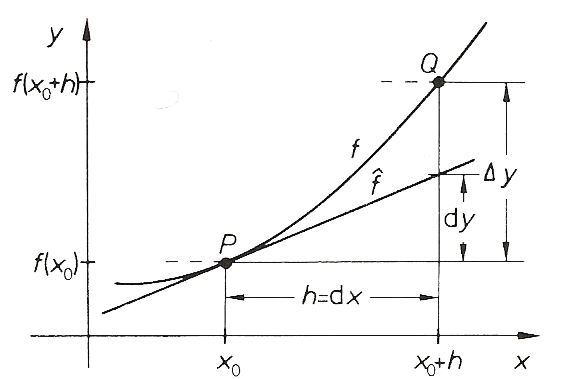
\includegraphics[width=5cm]{./bilder/differential_fehlerrechnung.png} 
	\end{minipage}
	\begin{minipage}[c]{13cm} 
		absoluter Fehler: $\left| \Delta y \right|	\approx \left| dy \right|=\left|f'(\bar{x})\right|\cdot\left| dx \right| \leq	\left| f'(\bar{x}) \right| \cdot \left| \delta \right| $  \\
		relativer Fehler: $|\Delta y| \approx |\frac{dy}{y}| = |\frac{f'(x)}{y}| \cdot |dx| \leq |\frac{f'(x)}{y}| \cdot |\delta| = |\frac{f'(x)}{f(x)} \cdot |\delta|  $ \\
		$|\frac{dx}{x}| \hat{=}$relative Fehler Input$ \qquad |\frac{dy}{y}| \hat{=} $relative Fehler Output$ \qquad $Einheit$ = [1]$\\
		Auf n-Stellen nach dem Komma genau $\Rightarrow \mbox{absoluter Fehler: } \delta = \pm 0.5 \cdot 10^{-n}$ 
	\end{minipage}


\subsection{Mittelwertsatz\formelbuchyellow{453}}
	\begin{minipage}[c]{5cm} 
		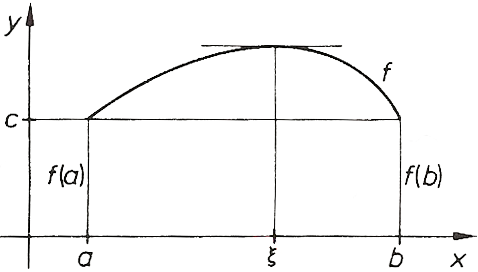
\includegraphics[width=3cm]{./bilder/differential_mittelwertsatz.png} 
	\end{minipage}
	\begin{minipage}[c]{7cm} 
		$\frac{\Delta y}{\Delta x}=\frac{f(b) - f(a)}{b - a} = f'(\xi) $ \\
		$\xi = a + \delta(b-a)$
	\end{minipage}
	\begin{minipage}[c]{5cm}
		$\frac{f(x+h) - f(x)}{h} = f'(x+\delta h)$\\
		$f(x+h) = h \cdot f'f(x+\delta h) + f(x)$ \\
		$\xi = x + \delta h \qquad 0<\delta<1$
	\end{minipage}	

\subsection{Taylor Polynom\formelbuchyellow{454,483}}
	($x_0$ = Entwicklungspunkt)$\quad f(x_0+h)=f(x_0) + f'(x_0)h + \frac{f''(x_0)}{2}h^2 + \frac{f'''(x_0)}{3!}h^3 + \ldots + \frac{f^{(n)}(x_0)}{n!}h^n + R_n(x_0, h)$\\
	$ h = x-x_0$\\
	$R_n$(Lagrange):$\quad R_n(x_0, h) = \frac{f^{(n+1)}(x_0 + \delta h)}{(n+1)!}h^{n+1}, (0 < \delta < 1);
	\qquad 
	\lim\limits_{n \to \infty} R_n(x_0, h) = 0 \Longrightarrow f(x_0+h) = \sum\limits_{n=0}^{\infty} \frac{f^{(n)}(x_0)}{n!}h^n$\\	
	\flushleft MacLaurinsche-Form (gilt f"ur $x_0=0, h=x $): $ f(x)=\sum\limits_{k=0}^{n} \frac{f^{(k)}(0)}{k!} \cdot x^k + R_n; 
	\qquad 
	R_n = \frac{f^{(n+1)}(\delta x)}{(n+1)!} \cdot x^{n+1}, (0 < \delta < 1);$
	
\subsubsection{Einige Reihen\formelbuchyellow{19,476,1073}}
		$\sin x = x - \frac{x^3}{3!} +  \frac{x^5}{5!} \mp ... + (-1)^{n-1} \cdot \frac{x^{2n-1}}{(2n-1)!} + $
		$ \overbrace{(-1)^n \cdot \frac{\cos(\vartheta x)}{(2n+1)!} \cdot x^{2n+1}}^{R_n} $\\
		$e^x =  1 + \frac{x}{1} + \frac{x^2}{2!} + ... + \frac{x^n}{n!} + $
		$ \frac{e^{\vartheta x}}{(n+1)!} \cdot x^{n+1} $\\
		$\ln (1+x) = x - \frac{x^2}{2} + \frac{x^3}{3} \mp ... + (-1)^{n-1} \cdot \frac{x^n}{n} + $
		$ \frac{(-1)^n}{(1+\vartheta x)^{n+1}} \cdot \frac{x^{n+1}}{n+1} $ 

\subsection{Bernoulli-de l'Hospital\formelbuchyellow{56}}
	${lim} _{x\downarrow x_{0}} \frac{f_{1}(x)}{f_{2}(x)} = {lim} _{x\downarrow x_{0}} \frac{f'_{1}(x)}{f'_{2}(x)} $, dies gilt f"ur: "`$\frac{0}{0}$"' 1. Regel, oder "`$\frac{\pm\infty}{\pm\infty}$"' 2. Regel;   Z"ahler und Nenner separat ableiten!

\subsubsection{Spezialf"alle}
	\begin{minipage}[c]{7cm} 
		$0 \cdot \pm \infty$ $\Rightarrow$ $\frac{f_1}{\frac{1}{f_2}} = \frac{0}{0}$ oder $\frac{f_2}{\frac{1}{f_1}} = \frac{\pm \infty}{\pm \infty}$
	\end{minipage}
	\begin{minipage}[c]{4cm} 
		$\infty - \infty$ $\Rightarrow$ $\frac{\frac{1}{f_2} - \frac{1}{f_1}}{\frac{1}{f_1 \cdot f_2}} $
	\end{minipage}
	\begin{minipage}[c]{7cm} 
		$ f^g:
		\left\{ 	
			\begin{array}{l} 
				1^\infty \\ 
				0^0 \\ 
				\infty^0 
			\end{array} 
		\right\} =
	  e^{g \cdot ln(f)} =
		\left\{ 
			\begin{array}{l} 
				e^{\infty \cdot 0} \\ 
				e^{0 \cdot -\infty} \\ 
				e^{0 \cdot \infty}
			\end{array}
		\right\} $
	\end{minipage}	

\subsection{Kurvenuntersuchungen\formelbuchyellow{260}}
\begin{enumerate}
	\item Definitionsbereich\formelbuchyellow{48} $D_f$ und Absch"atzung des Wertebereichs $W_f$, wenn m"oglich anhand der Extremalstellen
	\item Symmetrie und Periodizit"at\formelbuchyellow{52}
	\item Nullstellen
	\item Stetigkeit\formelbuchyellow{59} und Differenzierbarkeit\formelbuchyellow{443} (Berechnung der Ableitungen)
	\item Extremwerte, Wendepunkte und Wendetangenten, Monotonie, Kr"ummungsverhalten\formelbuchyellow{51}
	\item Grenzwertaussagen (Asymptote, Pole, Verhalten von $f$ am Rande des Definitionsbereichs)
\end{enumerate}

\subsubsection{Monotonie\formelbuchyellow{452}}
\begin{tabular}{|c|c|c|c|c|l|}
	\hline $f'(x)$ & $f''(x)$ & $f'''(x)$ & $f^{(n-1)}(x)$ & $f^{(n)}$ & Funktion $f$ \\
	\hline $\geq 0$ & & & & & monoton wachsend\\
	\hline $> 0$ & & & & & streng monoton wachsend\\
	\hline $\leq 0$ & & & & & monoton fallend \\
	\hline $< 0$ & & & & & streng monoton fallend\\
	\hline $= 0$ & $= 0$ & $= 0$ & $\dots = 0$ & $> 0$ & streng monoton wachsend (falls $n$ ungerade)\\
	\hline $= 0$ & $= 0$ & $= 0$ & $\dots = 0$ & $< 0$ & streng monoton falls (falls $n$ ungerade) \\\hline
\end{tabular}

\subsubsection{Extremstelle\formelbuchyellow{455}}
\begin{tabular}{|c|c|c|c|c|l|}
	\hline $f'(x)$ & $f''(x)$ & $f'''(x)$ & $f^{(n-1)}(x)$ & $f^{(n)}$ & Funktion $f$ \\
	\hline $= 0$ & $> 0$ & & & & relatives Minimum, \textbf{Randstellen beachten}\\
	\hline $= 0$ & $< 0$ & & & & relatives Maximum, \textbf{Randstellen beachten}\\
	\hline $= 0$ & $= 0$ & $= 0$ & $\dots = 0$ & $> 0$ & relatives Minimum (falls $n$ gerade), \textbf{Randstellen beachten}\\
	\hline $= 0$ & $= 0$ & $= 0$ & $\dots = 0$ & $< 0$ & relatives Maximum (falls $n$ gerade), \textbf{Randstellen beachten}\\
	\hline\multicolumn{6}{|l|}{\textbf{Zweite Variante}  Falls bei $f'(x)$ an der Stelle $x_0$ ein Vorzeichenwechsel besteht, existiert dort eine Extremstelle} \\\hline
\end{tabular}

\subsubsection{Konvexit"at - Kr"ummungsverhalten\formelbuchyellow{253}}
\begin{tabular}{|c|c|c|c|c|l|}
	\hline $f'(x)$ & $f''(x)$ & $f'''(x)$ & $f^{(n-1)}(x)$ & $f^{(n)}$ & Funktion $f$ \\
	\hline & $\geq 0$ & & & & konvex (linksgekr"ummt)\\
	\hline & $> 0$ & & & & streng konvex (linksgekr"ummt)\\
	\hline & $\leq 0$ & & & & konkav (rechtsgekr"ummt)\\
	\hline & $< 0$ & & & & streng konkav (rechtsgekr"ummt)\\\hline
\end{tabular}

\subsubsection{Wendepunkte (Terassenpunkt)\formelbuchyellow{255}}
\begin{tabular}{|c|c|c|c|c|l|}
	\hline $f'(x)$ & $f''(x)$ & $f'''(x)$ & $f^{(n-1)}(x)$ & $f^{(n)}$ & Funktion $f$ \\
	\hline\ & $= 0$ & $\neq 0$ & & & Wendepunkt\\
	\hline $= 0$ & $= 0$ & $\neq 0$ & & & Terassen- oder Sattelpunkt\\
	\hline\multicolumn{6}{|l|}{\textbf{Zweite Variante}  Falls bei $f''(x)$ an der Stelle $x_0$ ein Vorzeichenwechsel besteht, existiert dort ein Wendepunkt} \\\hline
\end{tabular}

\subsubsection{Asymptote\formelbuchyellow{259}}
	Die Asymptote existiert nur wenn alle drei eigentlichen Grenzwerte existieren.
	F"ur Funktionen, die nicht gebrochenrational sind, kann die Asymptote wie folgt bestimmt werden. \\
	\ \\ %Leerzeile
 	Asymptote  $g: y = ax + b \Rightarrow \lim\limits_{x \rightarrow \infty}(f(x) - ax - b) = 0$\\
	\ \\ %Leerzeile
	$a = \lim\limits_{x \rightarrow \infty} \frac{f(x)}{x} $ oder $a = \lim\limits_{x \rightarrow \infty} f'(x) \qquad $\\
	gilt jedoch nur wenn in der ersten Formel die Bedingung f"ur Bernoulli-de l'Hospital erf"ullt sind.\\
	$b = \lim\limits_{x \rightarrow \infty} (f(x) - ax) $\\
	\ \\ %Leerzeile
	Dies alles gilt sinngem"ass auch f"ur $x \rightarrow -\infty$\\
	\ \\ %Leerzeile	
	Spezialfall: Wenn $\lim\limits_{x \rightarrow \infty} f(x)$ existiert, so ist $a = 0$ und $b = \lim\limits_{x \rightarrow \infty} f(x)$.
	
\subsection{Schnittwinkel von zwei Funktionen}
	\begin{enumerate}
		\item Bei einem Schnittpunkt gilt: $f(x)=g(x)$
		\item Schnittpunkt $S(x_0,y_0)$ berechnen
		\item Falls dies eine kubische Gleichung ist, den Wert durch ausprobieren herausfinden (Bereich von $-3 \dots 3$)
		\item Funktionen ableiten: $f'(x)$ und $g'(x)$
		\item Steigungen berechnen: $f'(x_0)=m_1$ und $g'(x_0)=m_2$
		\item Schnittwinkel mit Hilfe dieser Gleichung berechnen: $tan(\sigma)=\frac{m_2-m_1}{1+m_1m_2}$
	\end{enumerate}
	
\subsubsection{Normale}
	Wenn eine Normale zur Tangente berechnet werden muss gilt: $m_1*m_2=-1$
%%%%%%%%%%%%%%%%%%%%%%%%%%%%%%%%%%%%%%%%%%%%%%%%%%%%%%%%%%%%%%%%%%%%%%%%%%%%%%%%%%%%%%%%%%%%%%%%
% Integral 
%%%%%%%%%%%%%%%%%%%%%%%%%%%%%%%%%%%%%%%%%%%%%%%%%%%%%%%%%%%%%%%%%%%%%%%%%%%%%%%%%%%%%%%%%%%%%%%%
\section{Integralrechnung\formelbuchviolet{492}}

\subsection{Bestimmtes Integral\formelbuchviolet{505}}
  $I = \int\limits_{a}^{b}{f(\widetilde{x})}d\widetilde{x} = \lim\limits_{d(Z) \rightarrow 0}S(Z) = \lim\limits_{d(Z) \rightarrow 0}O(Z)  = \lim\limits_{d(Z) \rightarrow 0}U(Z)  $ \\ 
	$x$: Integrationsver"anderliche, $f$: Integranden, $[a,b]$: Integrationsintervall, $a/b$: untere bzw. obere Integrationsgrenze

\subsection{Integrierbarkeit}
	\begin{minipage}[c]{10cm}
		\begin{center}
			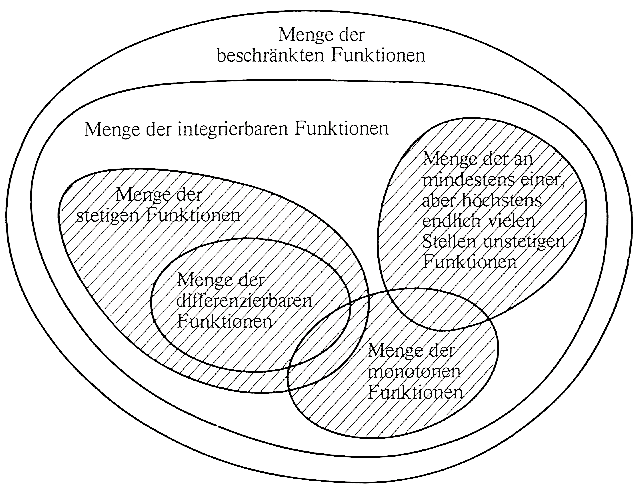
\includegraphics[width=6cm]{./bilder/integral_mengen.png} 
		\end{center}
	\end{minipage}
	\begin{minipage}[c]{7cm}
		\textbf{Schranken vom Integral:}\\
		$g_1(x) \leq f(x) \leq g_2(x)$\\
		$\int\limits_{a}^{b} g_1(\widetilde{x}) d\widetilde{x} \leq \int\limits_{a}^{b} f(\widetilde{x}) d\widetilde{x} \leq \int\limits_{a}^{b} g_2(\widetilde{x}) d\widetilde{x}$
	\end{minipage}
	
\subsection{Integralregeln\formelbuchviolet{494}}
	$\int\limits_a^b \widetilde{x}^n d\widetilde{x}=\frac{1}{n+1}(b^{n+1}-a^{n+1})$
	
\subsection{Fl"acheninhalt\formelbuchviolet{507}}
	Inhalt der Fl"ache unter dem Graphen $f: A = \int\limits_a^b |f(\widetilde{x})| d\widetilde{x}$ \\
	$A = A_1 - A_2 = \int\limits_a^b f_1(\widetilde{x}) d\widetilde{x} - \int\limits_a^b f_2{\widetilde{x}} d\widetilde{x} \qquad \text{gilt auch wenn die Funktionen }f_1 \text{ oder }f_2 \text{ negativ werden.}$

\subsection{Mittelwertsatz\formelbuchviolet{509}}
	$f$ auf $[a,b] \mbox{ stetig} \Rightarrow \mbox{ mind. eine Stelle } \xi \in (a,b)\mbox{ mit } \int\limits_a^b{f(\widetilde{x})}d\widetilde{x}=(b-a)f(\xi) 
	\Rightarrow h = \frac{1}{b-a} \int\limits_a^b{f(\widetilde{x})}d\widetilde{x}$ \\
	$h \hat{=}$ Mittelwert der Funktion

\subsection{Integralfunktion}
	$c \in [a,b]$ und $f(x)$ "uber $[a,b]$ integrierbar: $I: x \mapsto I(x) = \int\limits_c^x{f(\widetilde{t})}d\widetilde{t}$
	
\subsubsection{Differenzierbarkeit\formelbuchviolet{508}} 
	\begin{minipage}[t]{9.5cm}		
			$ \frac{d}{dx} \int\limits_{a(x)}^{b(x)} f(\widetilde{t}) d\widetilde{t} = f(b(x)) \cdot b'(x) - f(a(x)) \cdot a'(x) $
	\end{minipage}
	\begin{minipage}[t]{5cm} 	
			$ \qquad \frac{d}{dx} \int\limits_c^x f(\widetilde{t})d\widetilde{t} = f(x)$
	\end{minipage}
	
\subsection{Unbestimmtes Integral\formelbuchviolet{492}}
	$F(x) + C = \int{f(\widetilde{x})}d\widetilde{x}$

\subsection{Stammfunktion\formelbuchviolet{492}}
	Jede auf $[a,b]$ differenzierbare Funktion $F$ nennt man Stammfunktion, wenn $F'=f$.\\
	$I(x) \subset F(x)$

\subsection{Rechenregeln\formelbuchviolet{495}}
	\begin{tabular}{l c}
		$\int\limits_a^b f(\widetilde{x}) d\widetilde{x} = F(b) - F(a)$ & $|\int\limits_a^b f(x) dx| \leq \int\limits_a^b |f(\widetilde{x})| d\widetilde{x}$\\
		$\int\limits_a^b f(\widetilde{x}) d\widetilde{x} = \int\limits_0^b f(\widetilde{x}) d\widetilde{x} - \int\limits_0^a f(\widetilde{x})d\widetilde{x} = \int\limits_0^b f(\widetilde{x}) d\widetilde{x} - (-1) \cdot \int\limits_a^0 f(\widetilde{x})d\widetilde{x}$
	\end{tabular}



%\section{Zusatz}
%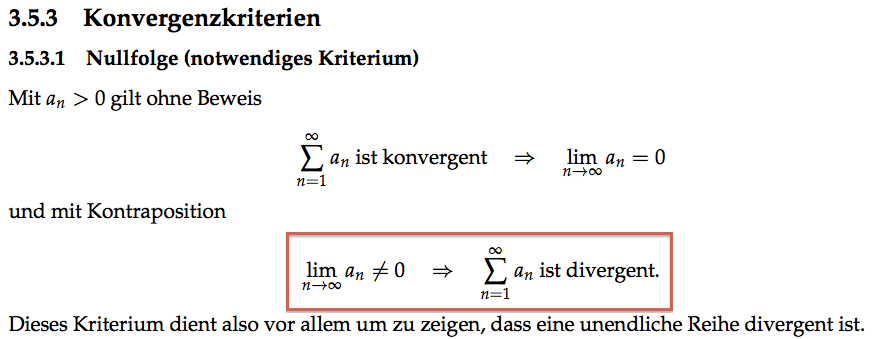
\includegraphics[width=8cm]{./bilder/konvergenzkriterien_nullfolge.png}  \\[10pt]
%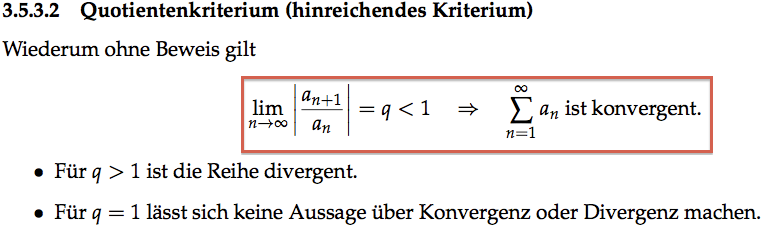
\includegraphics[width=8cm]{./bilder/konvergenzkriterien_quotientenkriterium.png}  \\[10pt]
%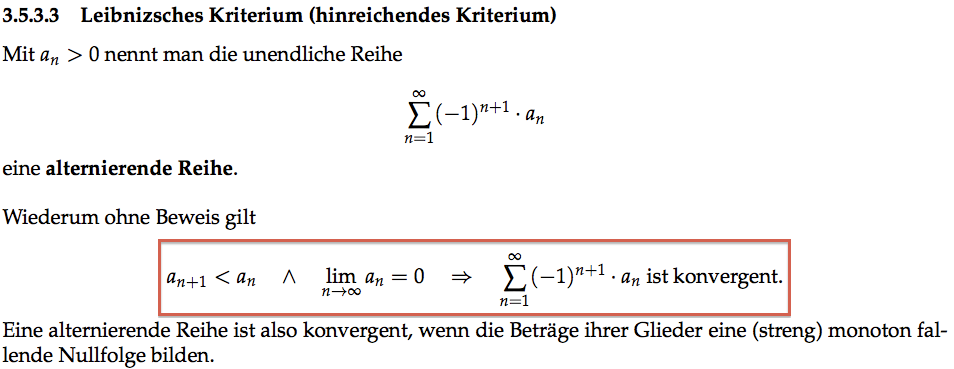
\includegraphics[width=10cm]{./bilder/konvergenzkriterien_Leibnizsches_Kriterium.png} \\ 
%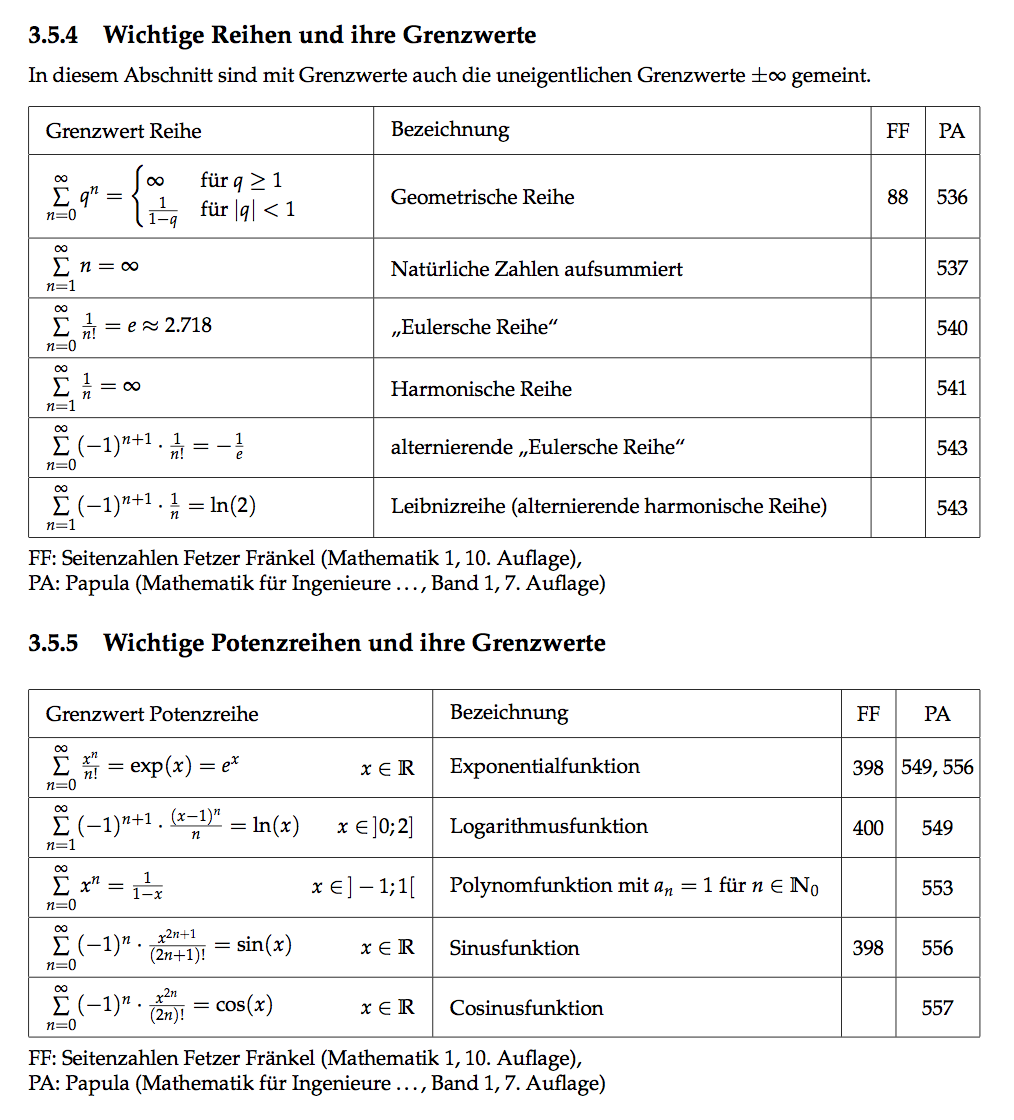
\includegraphics[width=12cm]{./bilder/wichtige_reihen_und_grenzwerte.png}  

\end{document}